\documentclass{beamer}
%% Possible paper sizes: a0, a0b, a1, a2, a3, a4.
%% Possible orientations: portrait, landscape
%% Font sizes can be changed using the scale option.
\usepackage[size=a1,orientation=landscape,scale=1.9]{beamerposter}
\usetheme{LLT-poster}
% \usecolortheme{ComingClean}
\usecolortheme{Entrepreneur}
% \usecolortheme{ConspiciousCreep}  %% VERY garish.

\usepackage[utf8]{inputenc}
\usepackage[T1]{fontenc}
\usepackage{libertine}
\usepackage[scaled=0.92]{inconsolata}
\usepackage[libertine]{newtxmath}

\usepackage{mwe}

\author[https://github.com/ShashankRao17/SOEN6011-Software-Engineering-Processes]{Shashank Rao - 40104247}
\title{\LARGE SOEN 6011: SOFTWARE ENGINEERING PROCESSES\\(\underline{Function F1 : ArcCos(x)})}
\institute{Concordia University - DEPARTMENT OF COMPUTER SCIENCE AND SOFTWARE ENGINEERING }
% Optional foot image
\footimage{
\includegraphics[width=14cm]{concordia_logo.png}}

\begin{document}
\begin{frame}[fragile]
\begin{columns}[T]

%%%% First Column
\begin{column}{.27\textwidth}

\begin{block}{Overview}
\begin{itemize}
\item Java application to obtain an angle(in degrees \& radians) for the inverse of cosine.
\item \large ArcCos $\theta$ = \Large$\frac{hypotenuse}{adjacent}$
\end{itemize}
\end{block}



\begin{block}{Domain \& Range of ArcCos(x)}
\begin{itemize}
\item The domain of $y=arccos(x)$ is the range of $f(x)=cos(x)$ for 0$\leq$x$\leq$$\pi$ and given by the interval \textbf{[-1,1]}. The range of arccos(x) is the domain of f which is given by the interval [0,$\pi$].

\end{itemize}
\end{block}

\begin{block}{Critical Decisions}
To ensure accuracy of output, the following decisions were critical:
\begin{itemize}
\item Use of \textbf{Taylor series expansion formula} instead of the Chebyshev-Pade quotient approximation:\\
$arccos(x)=\frac{\pi}{2}-\sum_{n=0}^{\infty}\frac{2n!}{2^{2n}(n!)^2}\frac{x^{2n+1}}{2n+1}$ which converges for -1$\leq$x$\leq$1.
    \begin{itemize}
        \item This decision was taken to avoid any static constants and to use a combination of iterative and recursive loops.
        \item Avoid declaration of multiple static constants(Chebyshev-Pade quotient approximation) thereby increasing complexity.
        \item Distribution of various critical functions into separate methods to adhere to Object Oriented Principles of Java.
    \end{itemize}

\end{itemize}
\end{block}

\end{column}

%%%% Second Column
\begin{column}{.3\textwidth}

\begin{block}{Arccos Table - Some of the commonly known values}
\begin{center}
		\begin{tabular}{|c|c|c|}
			\hline
			x&arccos(x)&arccos(x)\\
			 &(Rad)&($^{\circ}$)\\
			 \hline
			 -1&3.1413926536&180$^{\circ}$\\
			 \hline
			 -$\sqrt{3}$/2&2.6178432893&150$^{\circ}$\\
			 \hline
			 -$\sqrt{2}$/2&2.3560849003&135$^{\circ}$\\
			 \hline
			 -1/2&2.0942951024&120$^{\circ}$\\
			 \hline
			 0&1.5706963268&90$^{\circ}$\\
			 \hline
			1/2&1.0471977682&60$^{\circ}$\\
			 \hline
			 $\sqrt{2}$/2&0.7854077535&45$^{\circ}$\\
			 \hline
			 $\sqrt{3}$/2&0.5236495809&30$^{\circ}$\\
			 \hline
			 1&0.0&0$^{\circ}$\\
			 \hline
		\end{tabular}
	\end{center}
\end{block}

\begin{block}{Application User Interface}
    \begin{center}
        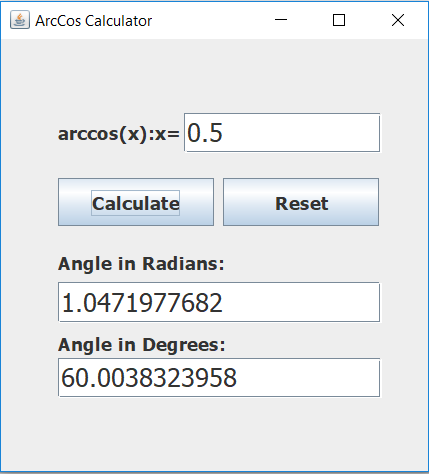
\includegraphics[width=.60\columnwidth]{working.PNG}
    \end{center}
\end{block}
\end{column}

%%%% This is the THIRD column
\begin{column}{.35\textwidth}
\begin{block}{Application User Interface - Error Handling}
\begin{center}
    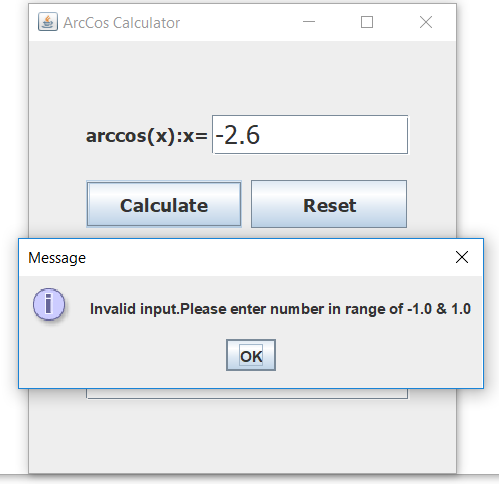
\includegraphics[width=.60\columnwidth]{NotWorking_negative_input.PNG}
\end{center}
\end{block}

\begin{block}{Conclusion}
\begin{itemize}
    \item The Java program/application contains all the key quality attributes such as: \textit{Correctness, Efficiency, Maintainability, Robustness and Usability}. 
    \item Due to the selection of the \textit{Taylor series expansion formula} for implementation of the $arccos(x)$ function, the accuracy of output is better with error coefficient $\approx$ 0.001 to 0.003 off the actual value.
\end{itemize}
\end{block}

\begin{block}{References}
\begin{itemize}
    \small\item https://www.mathportal.org/formulas/pdf/taylor-series-formulas.pdf
    \small\item https://en.wikipedia.org/wiki/Inverse trigonometric functions
\end{itemize}
\end{block}

\end{column}

\end{columns}

\end{frame}
\end{document}